\documentclass[a4paper]{article}

\usepackage{authblk}
\usepackage{mathrsfs}
\usepackage{tikz}
\usepackage{hyperref}
\hypersetup{
  pdfauthor = {Nikolaos Pothitos},
  pdftitle = {Annual Report for the PhD Thesis "Constraint
              Programming: Algorithms and Systems"}
}

\begin{document}

\title{Annual Report for the PhD Thesis ``Constraint
       Programming: Algorithms and Systems''}

\author{Nikolaos Pothitos ($\Delta$541)}

\affil{\normalsize
       Department of Informatics and Telecommunications \\
       National and Kapodistrian University of Athens \\
       Panepistimiopolis, 157\,84 Athens, Greece \\
       pothitos@di.uoa.gr}

\date{Academic Year 2017--2018}

\maketitle

This dissertation is supervised by Prof.~Panagiotis
Stamatopoulos.


\section{Naxos Solver Development}

In the past academic year, we published our Constraint
Programming library \textsc{Naxos Solver} according to the
open source community standards~\cite{Naxos}.

Declarativity is a \textsc{Naxos} key feature and it has to
do with describing problems and search methods
independently. \textsc{Naxos} serves the Constraint
Programming principle: \emph{The user states the problem,
the computer solves it}~\cite{Freuder2014}.

It supports the definition of custom search methods via a
declarative API, which is outlined in the next section.


\section{Building Search Methods with Self-confidence}

This is the title of the journal article we already
submitted~\cite{Pothitos2017} as an extension of our
conference paper ``Piece of Pie Search: Confidently
Exploiting Heuristics''~\cite{Pothitos2016-PoPS}.

In the late 1990s, \emph{Constrained Programming} (CP)
promised to separate the declaration of a problem from the
process to solve it. We attempt to serve this direction, by
implementing and presenting a modular way to defile
\emph{search methods} that seek solutions to arbitrary
\emph{Constraint Satisfaction Problems} (CSPs). The user
just declares their CSP, and it can be solved using a
portfolio of search methods already in place.

We allow the user\slash programmer to state their own
\emph{search methods} that can apply to any CSP. We found a
framework where the user can compose their search methods
out of conjunctive and disjunctive goals.

\subsection{A Goal-driven Search Methods'
            Framework\label{framework}}

Except from a way to state CSPs, a user\slash programmer
needs an elegant way to state search methods that solve
them. The CSPs should be ``search-methods-agnostic,'' while
the search methods should be ``CSP-agnostic'' in order to
keep the independence between the Constraint Programming
stages.

In related works, a lot of search methods have been
implemented in modern solvers~\cite{Gecode}. However, in our
case we try to provide a transparent framework, so that the
user can easily define their own methods.

\subsubsection{Search methods are made up of goals}

Every constructive search method is built up of goals. Each
goal executes an operation, e.g.\ an assignment of a value
to a constrained variable. Optionally, one goal returns
another goal to be executed. The goal returned can be a
\emph{meta}-goal, that is a goal that refers to another two
goals. There are two meta-goal kinds:
\begin{enumerate}
  \item The $\mathsf{AND}(g_1,g_2)$, which implies that the
        two sub-goals $g_1$ and $g_2$ must be executed and
        succeed both.
  \item The $\mathsf{OR}(g_1,g_2)$, which executes $g_1$. If
        $g_1$ does not succeed, i.e.\ if it does not lead to
        a solution, then $g_2$ is executed.
\end{enumerate}
This goal-driven framework is able to describe most of the
common search methods.

\subsubsection{The Depth-First Search example}

An elementary search method that can be straightforwardly
described via goals is \emph{depth-first search} (DFS). This
method iterates through the variables of a CSP\@. For each
variable $X$ selected, it selects a value $v$ from its
domain and makes the assignment $X \gets v$. It subsequently
proceeds to the next unassigned variable and makes another
assignment, etc.

If every variable is assigned a value and no constraint is
violated, the assignments set consists a \emph{solution}. In
any case, if there is a constraint violated, the last
assignment to a variable is undone and we try to assign
another value from its domain. If all the alternative values
are exhausted, we \emph{backtrack} to the previous variable
selected and we undo its assignment and so forth.

\subsubsection{Defining DFS using goals\label{DFS-goals}}

The ultimate goal in DFS and in every constructive search
method is to \texttt{Label} every variable with a value.
Each \texttt{Label}'s call aims to \texttt{Instantiate} a
variable.
\begin{itemize}
  \item \texttt{Label}($\emptyset$) := \textsf{success}.
  \item \texttt{Label}($\mathscr{X}$) :=
          \textsf{AND}(\texttt{Instantiate}($X$),
            \texttt{Label}($\mathscr{X} \! - \! \{X\}$)),
        with $X \in \mathscr{X}$,
\end{itemize}
where $\mathscr{X}$ is the set of all the variables. While
\texttt{Label} iterates recursively through the CSP
variables, an \texttt{Instantiate} call attempts to assign a
selected value $v$ to the variable $X$. If the assignment
fails to produce a solution, the value $v$ is deleted and
another instantiation is attempted, until all the
alternatives in $D_X$ are exhausted.
\begin{itemize}
  \item \texttt{Instantiate}($X$) := \textsf{failure},
          with $D_X = \emptyset$.
  \item \texttt{Instantiate}($X$) :=
          \textsf{OR}($X \! \gets \! v$,
            \textsf{AND}($D_X \!\! \gets \!\!
            D_X \!\! - \!\! \{v\}$,\,
            \texttt{Instantiate}($X$))), with $v \in D_X$.
\end{itemize}
The interdependencies between the above DFS goals are
graphically displayed in Fig.~\ref{DFS}.

\begin{figure}
  \centering
  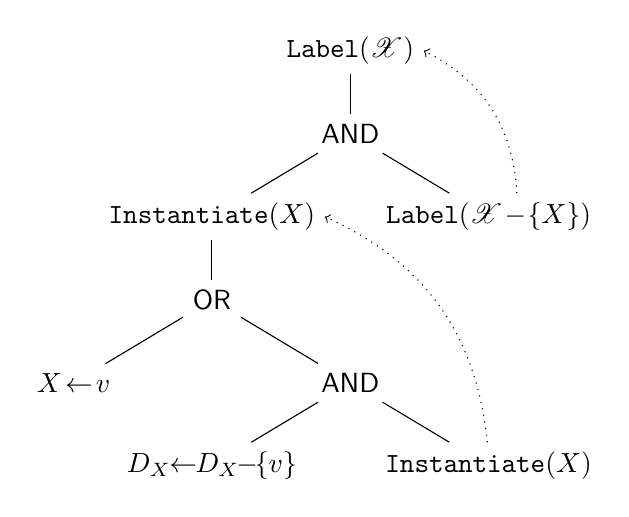
\begin{tikzpicture}
    [level distance = 3em, sibling distance = 10em,
     recursion/.style = {->, dotted, bend right}]
    \node (Label) {\texttt{Label}($\mathscr{X}$)}
      child {node {\textsf{AND}}
        child {node (Instantiate) {\texttt{Instantiate}($X$)}
          child {node {\textsf{OR}}
            child {node {$X \! \gets \! v$}}
            child {node {\textsf{AND}}
              child {node {$D_X \!\! \gets \!\! D_X \!\! - \!\! \{v\}$}}
              child {node (InstantiateChild) {\texttt{Instantiate}($X$)}}
            }
          }
        }
        child {node (LabelChild) {\texttt{Label}($\mathscr{X} \! - \! \{X\}$)}}
      };
    \path
      (LabelChild.40) edge [recursion] (Label.east)
      (InstantiateChild) edge [recursion] (Instantiate.east);
  \end{tikzpicture}
  \caption{The combination of the goals that compose
           DFS\label{DFS}}
\end{figure}


\section{Future Work}

In the current academic year we are going to investigate the
advantages of enforcing lightweight consistency levels into
constraint networks~\cite{Bessiere2006}.

\bibliographystyle{alpha}
\bibliography{bibliography}

\end{document}
